\begin{adjustbox}{max totalsize={\textwidth}{.9\textheight}, center}
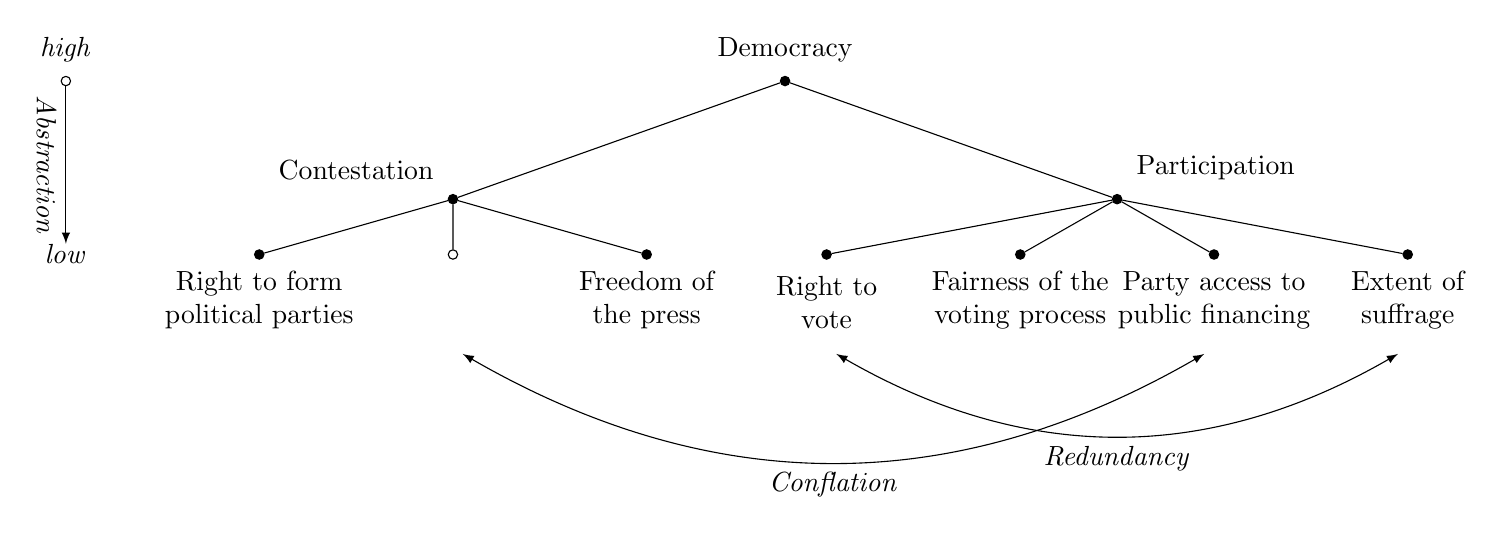
\begin{tikzpicture}[>=latex]
  % \usetikzlibrary{coordinates}
  \usetikzlibrary{positioning}
  \usetikzlibrary{calc}
% --- Layout & Styles --------------------------------------
\tikzstyle{solid node}=[circle,draw,inner sep=1.2,fill=black];
\tikzstyle{hollow node}=[circle,draw,inner sep=1.2];
\tikzstyle{level 1}=[sibling distance = 24em]
\tikzstyle{level 2}=[sibling distance = 7em, level distance = 2em]
% --- Tree -------------------------------------------------
\node(0)[solid node]{}
  child{
    node(0-1)[solid node]{}
      child{node(0-1-1)[solid node]{}}
      child{node(0-1-2)[hollow node]{}}
      child{node(0-1-3)[solid node]{}}
  }
  child{
    node(0-2)[solid node]{}
    child{node(0-2-1)[solid node]{}}
    child{node(0-2-2)[solid node]{}}
    child{node(0-2-3)[solid node]{}}
    child{node(0-2-4)[solid node]{}}
  }
  ;
\node [left=9 of 0, hollow node] (u) {};
\node [below=2 of u] (l) {};

% --- Node labels ------------------------------------------
\draw node at (0) [label = north:{Democracy}] {} ;
\draw node at (0-1) [label = north west:{Contestation}] {} ;
\draw node at (0-2) [label = north east:{Participation}] {} ;
\draw node [below=of 0-1-1, label = {[align=center]Right to form\\political parties}] {} ;
\draw node (b11) [below=of 0-1-2] {} ;
\draw node [below=of 0-1-3, label = {[align=center]Freedom of\\the press}] {} ;
\draw node (a11) [below=of 0-2-1, label = {[align=center]Right to\\vote}] {} ;
\draw node [below=of 0-2-2, label = {[align=center]Fairness of the\\voting process}] {} ;
\draw node (b12) [below=of 0-2-3, label = {[align=center]Party access to\\public financing}] {} ;
\draw node (a12) [below=of 0-2-4, label = {[align=center]Extent of\\suffrage}] {} ;
\draw node at (u) [label = north:{\textit{high}}] {};
\draw node at (l) {\textit{low}};


% --- Edges ------------------------------------------------
\draw [bend right, <->] (a11) to node [auto, below] {\textit{Redundancy}} (a12);
\draw [bend right, <->] (b11) to node [auto, below] {\textit{Conflation}}(b12) ;
\draw [->] (u) to node [auto, below, rotate=-90] {\textit{Abstraction}}(l) ;

\end{tikzpicture}
\end{adjustbox}
